\documentclass[12pt, a4paper]{article}

% Margins and Geometry
\usepackage[margin=1in]{geometry}

% Input Encoding
\usepackage[utf8]{inputenc}

% Math and Symbols
\usepackage{amsmath, amssymb}

% Graphics and Colors
\usepackage{tikz}
\usetikzlibrary{shapes, arrows.meta, positioning}
\usepackage{graphicx}
\usepackage[dvipsnames,table]{xcolor} % Using more color names, enable table features

% Tables
\usepackage{booktabs} % For professional looking tables
\usepackage{array} % For better column definitions
\usepackage{makecell} % Allows line breaks in cells

% Layout and Formatting
\usepackage{fancyhdr} % For headers and footers
\usepackage{titlesec} % To customize section titles
\usepackage{caption} % For captions outside floats
\usepackage{multicol} % For multi-column layout (optional)
\usepackage{parskip} % Adds space between paragraphs instead of indent

% Icons (Using fontawesome5 for more icons)
\usepackage{fontawesome5}

% Code Listing
\usepackage{listings} % For code blocks
\usepackage{tcolorbox} % For colored boxes around text/code
\tcbuselibrary{listings, skins, breakable} % Integrate tcolorbox with listings, skins and allow breaking

% Hyperlinks (Optional, but good for references)
% Load hyperref last with few exceptions (like cleveref)
\usepackage[hidelinks]{hyperref}


%-------------------------------------------------------------------------------
% Customization (Similar to Bresenham example)
%-------------------------------------------------------------------------------

% Page Style
\pagestyle{fancy}
\fancyhf{} % Clear header/footer
\lhead{\textcolor{RoyalBlue}{\faBookOpen~ Graphics Notes}}
\rhead{\textcolor{RoyalBlue}{\faBullseye~ Midpoint Circle Algorithm}} % Changed Icon & Title
\cfoot{\textcolor{gray}{Page \thepage}}
\renewcommand{\headrulewidth}{0.4pt} % Header rule
\renewcommand{\footrulewidth}{0.4pt} % Footer rule

% Section Title Formatting
\titleformat{\section}
  {\Large\bfseries\color{NavyBlue}} % Format
  {\color{NavyBlue}\faAngleRight~\thesection.} % Label
  {0.5em} % Horizontal separation
  {} % Code before title
  [\color{NavyBlue}\titlerule] % Code after title (adds a rule)

\titleformat{\subsection}
  {\large\bfseries\color{MidnightBlue}} % Format
  {\color{MidnightBlue}\faCaretRight~\thesubsection.} % Label
  {0.5em} % Horizontal separation
  {} % Code before title

% TikZ Style
\tikzstyle{point}=[circle, fill=blue, inner sep=1.5pt]
\tikzstyle{centerpoint}=[circle, fill=red, inner sep=1.5pt]
\tikzstyle{axis}=[->, >=Latex, thick, gray]
\tikzstyle{gridline}=[thin, gray!40]
\tikzstyle{dashedcircle}=[dashed, gray]

% Listings Style (for code blocks - same as before)
\lstdefinestyle{customcpp}{
  language=C++,
  basicstyle=\ttfamily\small,
  keywordstyle=\color{blue}\bfseries,
  stringstyle=\color{purple},
  commentstyle=\color{ForestGreen}\itshape,
  numbers=left,
  numberstyle=\tiny\color{gray},
  stepnumber=1,
  numbersep=5pt,
  backgroundcolor=\color{gray!10},
  showspaces=false,
  showstringspaces=false,
  showtabs=false,
  frame=tb, % Top and bottom frame
  framerule=0pt, % Frame rule width
  captionpos=b, % Caption position
  breaklines=true,
  breakatwhitespace=true,
  tabsize=2,
  morekeywords={uint32_t, GL_POINTS, glBegin, glEnd, glVertex2i} % Add OpenGL specific keywords
}

\lstdefinestyle{custompy}{
  language=Python,
  basicstyle=\ttfamily\small,
  keywordstyle=\color{blue}\bfseries,
  stringstyle=\color{purple},
  commentstyle=\color{ForestGreen}\itshape,
  numbers=left,
  numberstyle=\tiny\color{gray},
  stepnumber=1,
  numbersep=5pt,
  backgroundcolor=\color{gray!10},
  showspaces=false,
  showstringspaces=false,
  showtabs=false,
  frame=tb,
  framerule=0pt,
  captionpos=b,
  breaklines=true,
  breakatwhitespace=true,
  tabsize=2,
}

% tcolorbox setup for code (same as before)
\newtcblisting{cppcode}{
  listing engine=listings,
  listing only,
  breakable, % Allows the box to break across pages
  colback=gray!5,
  colframe=NavyBlue!75!black,
  title=\faCode~ C++ / OpenGL Implementation Snippet,
  fonttitle=\bfseries,
  listing options={style=customcpp},
  enhanced,
  overlay={\draw[NavyBlue!75!black,line width=0.5pt] ([yshift=-2pt]frame.south west)--([yshift=-2pt]frame.south east);} % Manual bottom rule inside box
}

\newtcblisting{pythoncode}{
  listing engine=listings,
  listing only,
  breakable, % Allows the box to break across pages
  colback=gray!5,
  colframe=OliveGreen!75!black,
  title=\faPython~ Python Implementation Snippet,
  fonttitle=\bfseries,
  listing options={style=custompy},
  enhanced,
  overlay={\draw[OliveGreen!75!black,line width=0.5pt] ([yshift=-2pt]frame.south west)--([yshift=-2pt]frame.south east);} % Manual bottom rule inside box
}

% Custom command for drawing symmetric points in TikZ (same as before)
\newcommand{\drawCirclePoints}[2]{
    \node[point] at (#1,#2) {}; \node[point] at (#2,#1) {};
    \node[point] at (-#1,#2) {}; \node[point] at (-#2,#1) {};
    \node[point] at (#1,-#2) {}; \node[point] at (#2,-#1) {};
    \node[point] at (-#1,-#2) {}; \node[point] at (-#2,-#1) {};
}

% Increase row spacing slightly for makecell
\renewcommand{\arraystretch}{1.3}
% Set default alignment for makecell to left & add padding
\setcellgapes{3pt}
\makegapedcells

%-------------------------------------------------------------------------------
% Document Start
%-------------------------------------------------------------------------------
\begin{document}

% Title Block
\begin{tcolorbox}[
    colback=RoyalBlue!10!white,
    colframe=RoyalBlue!75!black,
    sharp corners,
    boxrule=1pt,
    center title
    ]
    {\Huge \bfseries \faBullseye~ Midpoint Circle Drawing Algorithm} \\[0.2cm] % Changed Icon & Title
    {\large A Structured Study Note with Code Examples}
\end{tcolorbox}
\vspace{0.5cm}

% Quick Notes Section
\begin{tcolorbox}[
    colback=yellow!10!white,
    colframe=orange!75!black,
    title=\faStickyNote~ Quick Notes,
    fonttitle=\bfseries\large
    ]
    \begin{itemize}
        \item Also known as Bresenham's Circle Algorithm (the integer-only version is often derived via the midpoint approach).
        \item Efficiently draws circles on raster displays using primarily \textbf{integer arithmetic}.
        \item Evaluates the circle function at the \textbf{midpoint} between two candidate pixels to decide which pixel is closer to the ideal circle.
        \item Exploits \textbf{8-way symmetry} for performance, calculating points for only one octant.
    \end{itemize}
\end{tcolorbox}

\section{Initial Setup}
Similar to other incremental algorithms, we define the circle and starting parameters. We focus on the second octant (90 to 45 degrees).
\begin{itemize}
    \item Circle Center $(x_c, y_c) = (0, 0)$
    \item Radius $R$
    \item Starting Point: $(x_0, y_0) = (0, R)$
    \item Circle Function: $f(x, y) = x^2 + y^2 - R^2$. $f(x,y) < 0$ for points inside, $f(x,y) > 0$ for points outside.
    \item Initial Decision Parameter $p_0$: Evaluate $f(x, y)$ at the midpoint between the first two candidate pixels $(1, R)$ and $(1, R-1)$. The midpoint is $(1, R - \frac{1}{2})$.
    \[
        p_0 = f(1, R - \tfrac{1}{2}) = 1^2 + (R - \tfrac{1}{2})^2 - R^2 = 1 + R^2 - R + \tfrac{1}{4} - R^2 = \tfrac{5}{4} - R
    \]
    For integer-only arithmetic, we can define $p_k = f(x_k + 1, y_k - \frac{1}{2})$, which leads to an integer starting value:
    \[ p_0 = 1 - R \]
    (This common simplification effectively shifts the decision boundary slightly but produces the same pixel choices).
    \item \textbf{Example:} For $R = 5$:
    \[
        p_0 = 1 - 5 = -4
    \]
\end{itemize}

\section{Decision Parameter and Update Rules}
At each step $k$, starting with $(x_k, y_k)$, we consider the midpoint $M = (x_k+1, y_k - \frac{1}{2})$ between the next two candidate pixels: East $E = (x_k+1, y_k)$ and South-East $SE = (x_k+1, y_k-1)$. The decision parameter $p_k = f(M)$ determines which pixel is closer.

\begin{center}
\captionof{table}{Update Rules Based on Midpoint Decision Parameter $p_k$}
\label{tab:midpoint_update_rules}
\begin{tabular}{@{}c l c l@{}}
\toprule
\textbf{Condition} & \makecell[l]{\textbf{Midpoint Location}\\\textbf{(Relative to Circle)}} & \makecell[c]{\textbf{Next Point Chosen}\\\textbf{$(x_{k+1}, y_{k+1})$}} & \makecell[l]{\textbf{Update Rule}\\\textbf{for } $p_{k+1}$} \\
\midrule
$p_k < 0$ & Midpoint is inside & E = $(x_k+1, y_k)$ & $p_{k+1} = p_k + 2x_k + 3$ \\
\midrule
$p_k \geq 0$ & Midpoint is outside or on & SE = $(x_k+1, y_k-1)$ & $p_{k+1} = p_k + 2(x_k - y_k) + 5$ \\
\bottomrule
\end{tabular}
\end{center}
The calculation proceeds from $x=0$ and stops when $x \geq y$.

\section{Step-by-Step Calculation (Example: R=5)}
\textbf{Given:} $R = 5$, Center $(0, 0)$, Start Point $(0, 5)$, $p_0 = -4$.

\begin{center}
\captionof{table}{Midpoint algorithm calculation steps for R=5.}
\label{tab:midpoint_calc_steps}
\begin{tabular}{|c|c|c|c|c|l|}
\hline
\makecell{\textbf{Step}\\\textbf{(k)}} & \makecell[c]{\textbf{Current Point}\\\textbf{$(x_k, y_k)$}} & $p_k$ & \makecell{\textbf{$p_k < 0$?}} & \makecell[c]{\textbf{Next Point}\\\textbf{$(x_{k+1}, y_{k+1})$}} & \makecell[l]{\textbf{Calculation}\\\textbf{for } $p_{k+1}$} \\
\hline
0 & (0, 5) & -4 & Yes & (1, 5) & \makecell[l]{$p_1 = p_0 + 2x_0 + 3$ \\ $= -4 + 2(0) + 3 = -1$} \\
\hline
1 & (1, 5) & -1 & Yes & (2, 5) & \makecell[l]{$p_2 = p_1 + 2x_1 + 3$ \\ $= -1 + 2(1) + 3 = 4$} \\
\hline
2 & (2, 5) & 4 & No & (3, 4) & \makecell[l]{$p_3 = p_2 + 2(x_2 - y_2) + 5$ \\ $= 4 + 2(2 - 5) + 5$ \\ $= 4 - 6 + 5 = 3$} \\
\hline
3 & (3, 4) & 3 & No & (4, 3) & \makecell[l]{$p_4 = p_3 + 2(x_3 - y_3) + 5$ \\ $= 3 + 2(3 - 4) + 5$ \\ $= 3 - 2 + 5 = 6$} \\
\hline
\multicolumn{6}{|c|}{\textbf{Stop:} $x=4, y=3 \implies x \ge y$} \\
\hline
\end{tabular}
\end{center}

The points generated in the second octant are: $(0, 5), (1, 5), (2, 5), (3, 4), (4, 3)$. (These are identical to the points generated by the Bresenham algorithm derivation used previously).

\section{Exploiting 8-Way Symmetry}
The Midpoint algorithm, like Bresenham's, calculates points for only one octant. The full circle is obtained by reflecting these points across the axes and diagonals ($y=x, y=-x$). If $(x, y)$ is a point calculated in the second octant (from $x=0$ to $x=y$), the following points are also on the circle:

\begin{center}
\captionof{table}{Mapping a Point $(x, y)$ to All 8 Octants (Same as Bresenham)}
\label{tab:midpoint_symmetry}
\rowcolors{2}{gray!15}{white} % Alternating row colors
\begin{tabular}{ccc}
\toprule
\textbf{Octant} & \textbf{Symmetric Point} & \textbf{Transformation from (x, y)} \\
\midrule
1 ($0^\circ-45^\circ$) & $(y, x)$ & Swap x and y \\
2 ($45^\circ-90^\circ$) & $(x, y)$ & Original point (calculated) \\
3 ($90^\circ-135^\circ$) & $(-x, y)$ & Negate x \\
4 ($135^\circ-180^\circ$) & $(-y, x)$ & Swap x and y, negate new x \\
5 ($180^\circ-225^\circ$) & $(-y, -x)$ & Swap x and y, negate both \\
6 ($225^\circ-270^\circ$) & $(-x, -y)$ & Negate both \\
7 ($270^\circ-315^\circ$) & $(x, -y)$ & Negate y \\
8 ($315^\circ-360^\circ$) & $(y, -x)$ & Swap x and y, negate new y \\
\bottomrule
\end{tabular}
\end{center}

\textbf{Applying Symmetry to R=5 Example Points:}\\
The calculated points $(0, 5), (1, 5), (2, 5), (3, 4), (4, 3)$ generate the same full set of circle points as shown in the Bresenham example when symmetry is applied.

\section{Visualization (TikZ)}

\begin{center}
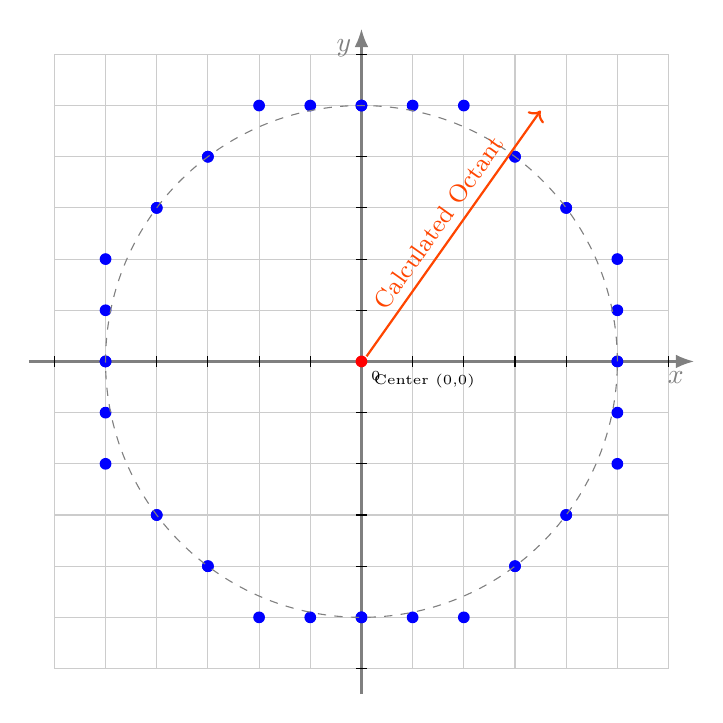
\begin{tikzpicture}[scale=0.65]
    % Grid
    \draw[gridline] (-6,-6) grid (6,6);

    % Axes
    \draw[axis] (-6.5,0) -- (6.5,0) node[below left] {$x$};
    \draw[axis] (0,-6.5) -- (0,6.5) node[below left] {$y$};

    % Origin Ticks
    \foreach \i in {-6,...,6} {
        \draw (\i, -0.1) -- (\i, 0.1);
        \draw (-0.1, \i) -- (0.1, \i);
    }
    \node[below right, font=\tiny] at (0,0) {0};

    % Center Point
    \node[centerpoint, label={[label distance=-1pt]below right:\tiny Center (0,0)}] at (0,0) {};

    % Calculated points and their symmetric counterparts
    % Points from calculation: (0,5), (1,5), (2,5), (3,4), (4,3)
    \drawCirclePoints{0}{5}
    \drawCirclePoints{1}{5}
    \drawCirclePoints{2}{5}
    \drawCirclePoints{3}{4}
    \drawCirclePoints{4}{3}

    % Dashed ideal circle
    \draw[dashedcircle] (0,0) circle (5);

    % Annotate one octant
    \draw[->, thick, OrangeRed] (0.1, 0.1) -- (3.5, 4.9) node[midway, above, sloped, font=\small] {Calculated Octant};
\end{tikzpicture}
\captionof{figure}{Plot of points for R=5 generated by the Midpoint Circle algorithm, showing 8-way symmetry.}
\label{fig:midpoint_tikz_circle}
\end{center}

\section{Code Implementations}

\subsection{C++ / OpenGL Snippet}
This snippet shows the Midpoint Circle algorithm logic. Assumes `drawPixel` and `drawCirclePoints` (for symmetry) exist as defined previously.

\begin{cppcode}
#include <GL/glut.h> // Or your preferred GL header

// Assumed: drawPixel(x, y) and drawCirclePoints(cx, cy, x, y) exist

// Midpoint Circle Drawing Algorithm
void drawCircleMidpoint(int cx, int cy, int r) {
    int x = 0;
    int y = r;
    int p = 1 - r; // Initial decision parameter (integer version)

    // Draw the first set of points based on the starting point (0, r)
    drawCirclePoints(cx, cy, x, y);

    // Calculate points for the second octant (from y-axis to y=x line)
    while (x < y) {
        x++; // Always increment x
        if (p < 0) {
            // Midpoint is inside, choose E pixel
            // Update p for the next E candidate: p_new = p + 2x_new + 1
            // Since x_new = x_old + 1, this is p + 2(x+1) + 1 = p + 2x + 3
            p = p + 2 * x + 3;
            // y remains the same
        } else {
            // Midpoint is outside or on the circle, choose SE pixel
            // Update p for the next SE candidate: p_new = p + 2x_new - 2y_new + 1
            // Since x_new = x+1, y_new = y-1, this is p + 2(x+1) - 2(y-1) + 1
            // p + 2x + 2 - 2y + 2 + 1 = p + 2(x - y) + 5
            y--; // Decrement y
            p = p + 2 * (x - y) + 5;
        }
        // Draw the calculated point and its symmetric counterparts
        drawCirclePoints(cx, cy, x, y);
    }
}

/*
// Example Usage in a GLUT display function:
void display() {
    glClear(GL_COLOR_BUFFER_BIT);
    glColor3f(0.0, 1.0, 0.0); // Set color to green

    glBegin(GL_POINTS); // Begin drawing points
    drawCircleMidpoint(0, 0, 50); // Draw circle at center (0,0) with radius 50
    glEnd(); // End drawing points

    glFlush();
}
*/
\end{cppcode}

\subsection{Python Snippet}
Python implementation of the Midpoint Circle algorithm.

\begin{pythoncode}
import matplotlib.pyplot as plt

def midpoint_circle_octant(r):
    """
    Calculates points for the second octant (90 to 45 degrees)
    using the Midpoint Circle algorithm. Starts at (0, r).
    """
    x = 0
    y = r
    p = 1 - r  # Initial decision parameter (integer version)
    points = []

    # Add the starting point
    points.append((x, y))

    # Iterate until x >= y (end of the octant)
    while x < y:
        x += 1
        if p < 0:
            # Select E point (x+1, y)
            p = p + 2 * x + 3
        else:
            # Select SE point (x+1, y-1)
            y -= 1
            p = p + 2 * (x - y) + 5

        points.append((x, y))

    return points

def get_symmetric_points(x, y):
    """Generates all 8 symmetric points for a given point (x, y)."""
    # (Same function as in Bresenham example)
    return [
        (x, y), (y, x), (-x, y), (-y, x),
        (x, -y), (y, -x), (-x, -y), (-y, -x)
    ]

def get_all_midpoint_circle_points(cx, cy, r):
    """
    Generates all points for a circle centered at (cx, cy) with radius r
    using the Midpoint algorithm.
    """
    octant_points = midpoint_circle_octant(r)
    all_points = set() # Use a set to avoid duplicates

    for x, y in octant_points:
        symmetric = get_symmetric_points(x, y)
        for sx, sy in symmetric:
            # Translate points relative to the center (cx, cy)
            all_points.add((cx + sx, cy + sy))

    return list(all_points)

# --- Example Usage ---
radius = 5
center_x = 0
center_y = 0

# Calculate points for the second octant
octant2_points_midpoint = midpoint_circle_octant(radius)
print(f"Points in the second octant (Midpoint, R={radius}): {octant2_points_midpoint}")

# Calculate all points for the circle
circle_points_midpoint = get_all_midpoint_circle_points(center_x, center_y, radius)
print(f"\nTotal unique points for the circle (Midpoint): {len(circle_points_midpoint)}")
# print(f"All points: {sorted(list(circle_points_midpoint))}") # Uncomment to see all points

# --- Optional: Plotting with Matplotlib ---
def plot_circle(points, title_suffix=""):
    if not points:
        print("No points to plot.")
        return

    x_coords, y_coords = zip(*points) # Unzip points into x and y lists

    plt.figure(figsize=(6, 6))
    plt.scatter(x_coords, y_coords, color='green', s=10) # Plot points (green)
    plt.axhline(0, color='grey', lw=0.5)
    plt.axvline(0, color='grey', lw=0.5)
    plt.grid(True, linestyle='--', alpha=0.6)
    plt.gca().set_aspect('equal', adjustable='box') # Ensure aspect ratio is equal
    plt.title(f"Midpoint Circle Points{title_suffix} (R={radius}, Center=({center_x},{center_y}))")
    plt.xlabel("X-axis")
    plt.ylabel("Y-axis")
    # Set limits slightly larger than radius
    lim = radius + 1
    plt.xlim(-lim, lim)
    plt.ylim(-lim, lim)
    plt.show()

# Plot the calculated points
# plot_circle(circle_points_midpoint, title_suffix=" - Midpoint") # Requires matplotlib

\end{pythoncode}

\section{Summary}
\begin{tcolorbox}[
    colback=Green!10!white,
    colframe=ForestGreen!75!black,
    title=\faCheckCircle~ Key Takeaways,
    fonttitle=\bfseries\large
    ]
    \begin{itemize}
        \item The Midpoint Circle Algorithm is another highly efficient, integer-based method for rasterizing circles.
        \item It explicitly uses the midpoint between candidate pixels to make decisions based on the circle equation $f(x,y)=x^2+y^2-R^2$.
        \item The resulting pixel coordinates and the update logic (using integer parameters) are often identical to those derived from Bresenham's approach.
        \item Like Bresenham's, it relies heavily on 8-way symmetry to minimize calculations.
    \end{itemize}
\end{tcolorbox}

\end{document}
